\documentclass[tikz,border=2pt]{standalone}

\usepackage[utf8]{inputenc}
\usepackage{pgf}
\usepackage{tikz}
\usetikzlibrary{arrows,automata}

\begin{document}

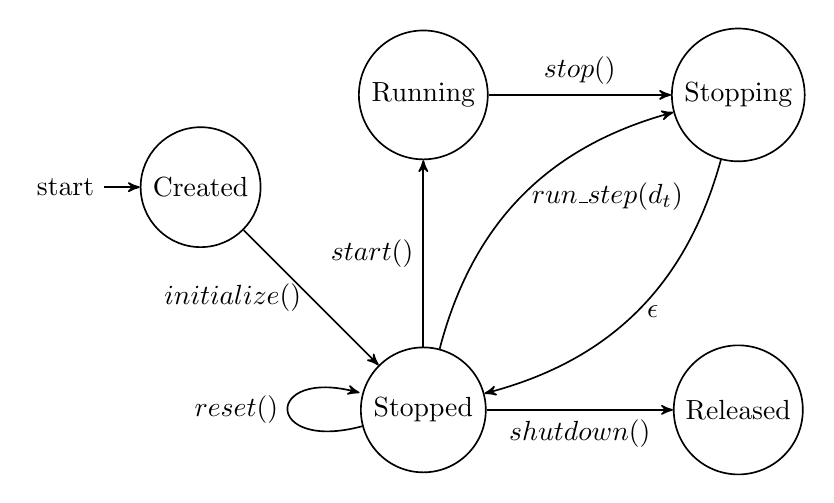
\begin{tikzpicture}[->,>=stealth',auto,semithick,node distance=4cm]

	\node[initial,state] (created) {Created};
	\node[state]         (stopped) [below right of=created]{Stopped};
	\node[state]         (started) [above of=stopped]{Running};
	\node[state]				 (stop)		 [right of=started]{Stopping};
	\node[state]  			 (shutdown)[right of=stopped]{Released};
	
	\path (created) 		edge node [left] {$initialize()$} (stopped)
				(stopped)			edge [bend left] node [right] {$run\_step(d_t)$} (stop)
											edge [loop left] node {$reset()$} (stopped)
											edge node{$start()$} (started)
											edge node [below] {$shutdown()$} (shutdown)
				(started)			edge node[above]{$stop()$} (stop)
				(stop)				edge [bend left] node[right]{$\epsilon$} (stopped);

\end{tikzpicture}

\end{document}
